\documentclass{article}
\usepackage[utf8]{inputenc}

\title{Handbook Code Implementation}
\author{Bernardo Fichera}
\date{November 2018}

\usepackage{natbib}
\usepackage{graphicx}

%=============================================%
% PERSONAL LATEX SETTING                      %
%=============================================%

% Packages
\usepackage{pgfplots} % Nice plots; loads tikz as well.
\usepackage{soul}
\usepackage{textcomp}
\usepackage{amssymb}
\usepackage{amsfonts}
\usepackage{amsmath}
\usepackage{mathrsfs}
\usepackage{mathtools}
\usepackage{subfig}
\usepackage{hhline}
\usepackage{array}
\usepackage{amsthm}
\usepackage{asymptote}
\usepackage{bm} % Bold works for greek letters too.
\usepackage{listings} % To write some code in the text.

% Options
\pgfplotsset{width=7cm,compat=1.10}
\usepgfplotslibrary{groupplots}
\usetikzlibrary{decorations.text,calc,arrows.meta, backgrounds}
\tikzset{image/.style={
    above right,
    inner sep=0pt,
    outer sep=0pt}
    }

% Commands
\DeclarePairedDelimiter\abs{\lvert}{\rvert}
\DeclarePairedDelimiter\norm{\lVert}{\rVert}
\DeclarePairedDelimiter\dprod{\langle}{\rangle}
% Swap the definition of \abs* and \norm*, so that \abs
% and \norm resizes the size of the brackets, and the 
% starred version does not.
\makeatletter
\let\oldabs\abs
\def\abs{\@ifstar{\oldabs}{\oldabs*}}
%
\let\oldnorm\norm
\def\norm{\@ifstar{\oldnorm}{\oldnorm*}}
%
\let\olddprod\dprod
\def\dprod{\@ifstar{\olddprod}{\olddprod*}}
\makeatother
%
\newcolumntype{C}[1]{>{\centering\arraybackslash}m{#1}}

% Math definitions
\newtheorem*{definition}{Definition}
\newtheorem*{proposition}{Proposition}
\newtheorem*{theorem*}{Theorem}
\newtheorem{theorem}{Theorem}[section]
\newtheorem*{corollary}{Corollary}
\newtheorem{lemma}[theorem]{Lemma}

% Figures path
\graphicspath{{pics/}}
%===================================================%

\begin{document}

\maketitle

\section*{Kernels}
In this section are listed the kernels adopted and the techniques used for the vectorized implementation. If you have two data set of different dimension reprensetd by matrices $X \in (m, d)$ and $Y \in (n\times d)$ you can query the kernel passing directly the data set:
\begin{equation*}
    k(X,Y) \rightarrow (m\times n, 1) 
\end{equation*}
This behavior is achieved by augmenting each data set as shown in figure \ref{fig:hbook1}.
\begin{figure}[ht]
    \centering
    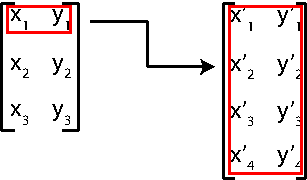
\includegraphics[width=.5\textwidth]{hbook_fig1.pdf}
    \caption{Vectors ordering.}
    \label{fig:hbook1}
\end{figure}
The first matrices is repeated $n$ times (number of data in $Y$) and each row wise element of $Y$ is repeated $m$ times (number of data in $X$).

\subsection*{RBF Kernel}
Kernel shape:
\begin{equation*}
    k(x,y) = e^{\frac{-\norm{x-y}^2}{2 \sigma^2}},
\end{equation*}
where $x,y \in \mathrm{R}^d$.
The kernel operates on the data matrices evaluating the norm of the difference between the first element of $X$ and, one by one, all the elements of $Y$; then the exponential decaying is applied. 


\begin{lstlisting}[frame=single]
X = repmat(x,size(y,1),1);
Y = repelem(y,size(x,1),1)
norm = vecnorm(X-Y,2,2)
exp(-norm.^2/2/sigma^2);
\end{lstlisting}
The pseudo code shows briefly the algorithm for MATLAB. 
\begin{itemize}
    \item \textbf{Querying name:} 'gauss'
    \item \textbf{Source name:} rbf.m
    \item \textbf{Required params:} $\sigma$
\end{itemize}

\begin{equation*}
    \sum_{k=1}^{m} \sum_{j=1}^{m} \alpha_k \alpha_j K_{kj} = \alpha_k K_k^i \alpha_j K_i^j = \alpha^T K \alpha
\end{equation*}

\begin{equation*}
    \sum_{i=1}^{m} \sum_{k=1}^{m} \alpha_k K_{ki} \sum_{j=1}^{m} \alpha_j K_{ij} = \alpha^T K^2 \alpha
\end{equation*}

\begin{equation*}
    k(x_i,x) = e^{d\norm{x_i-x}^2}
\end{equation*}

\begin{equation*}
    \frac{\partial}{\partial x} k(x_i,x) = -2d(x_i-x)^T k(x_j,x)
\end{equation*}

\begin{equation*}
    \frac{\partial}{\partial^2 x} k(x_i,x) = 2d\left[I + 2d(x_i-x)(x_i-x)^T \right]k(x_j,x)
\end{equation*}

\begin{equation}
    \sum_{i=1}^{m}\left( \sum_{k=1}^m \alpha_k G_{ki} \sum_{j=1}^m \alpha_j G_{ij}^T \right)
\end{equation}

\begin{equation}
    \left( \sum_{k=1}^m \alpha_k G_{ki} \sum_{j=1}^m \alpha_j G_{ij}^T \right)
\end{equation}

\begin{lstlisting}[frame=single]
I = repmat(reshape(eye(size(x,2)),1,[]),size(x,1)*size(y,1),1)
Y = repelem(y,size(x,1),1)
norm = vecnorm(X-Y,2,2)
exp(-norm.^2/2/sigma^2);
\end{lstlisting}

\subsection*{RBF Kernel Compact}

\begin{equation}
    k(x_i,x_j)=
    \begin{cases}
    e^{\frac{-\norm{x_i-x_j}^2}{2\sigma^2}}, \quad \text{if } \norm{x_i-x_j} \le r \\
    0, \hspace{1.8cm} \text{otherwise.}
    \end{cases}
\end{equation}

\subsection*{RBF Velocity Augmented}

\begin{equation}
k(\bm{\xi}_i,\bm{\xi}_j) = \left(1 + \lambda e^{\frac{-\norm{\bm{f}(\bm{\xi}_i)}^2}{\epsilon}}\right)e^{-\frac{\norm{\bm{\xi}_i-\bm{\xi}_j}^2}{2\sigma^2}}.
\end{equation}

\begin{equation}
k(\bm{\xi}_i,\bm{\xi}_j) = \left(1 + \lambda e^{\frac{-\norm{\bm{f}(\bm{\xi}_i)}^2}{\epsilon}}\right)e^{-\frac{\norm{\bm{\xi}_i-\bm{\xi}_j}^2}{2\sigma^2}}\left(1 + \lambda e^{\frac{-\norm{\bm{f}(\bm{\xi}_j)}^2}{\epsilon}}\right).
\end{equation}

\subsection*{RBF Attractors Augmented}
With
\begin{equation}
    k_{\sigma}(\bm{x}_i,\bm{x}_j) = e^{-\frac{\norm{\bm{x}_i-\bm{x}_j}^2}{2\sigma^2}},
\end{equation}
the attractors augmented kernel is
\begin{equation*}
k(\bm{x}_i,\bm{x}_j) = \left(1 + \lambda \sum_a^A k_{\sigma}(\bm{x}_a,x_i)\right)k_{\epsilon}(\bm{x}_i,\bm{x}_j)\left(1 + \lambda \sum_a^A k_{\sigma}(\bm{x}_a,x_j)\right).
\end{equation*}

\subsection*{RBF Velocity Hyperparameter}
\begin{equation}
    k_{\sigma}(\bm{x}_i,\bm{x}_j) = e^{-\frac{\norm{\bm{x}_i-\bm{x}_j}^2}{2\norm{\dot{x}_i}^2}},
\end{equation}

\subsection*{Non-Stationary Anisotropic Kernel}

\begin{equation*}
    C^{NS}(x_i,x_j) = \sigma^2 \abs{\Sigma_i}^{\frac{1}{4}}\abs{\Sigma_j}^{\frac{1}{4}}\abs{\frac{\Sigma_i+\Sigma_j}{2}}^{-\frac{1}{2}} \exp{-Q_{ij}}
\end{equation*}

\begin{equation*}
    Q_{ij} = (x_i-x_j)^T \left( \frac{\Sigma_i+\Sigma_j}{2} \right)^{-1} (x_i-x_j).
\end{equation*}

\subsection*{Anisotropic Velocity-Oriented Kernel}


\subsection*{Lyapunov RBF Kernel}
With
\begin{equation}
    k_{\sigma}(\bm{x}_i,\bm{x}_j) = e^{-\frac{\norm{\bm{x}_i-\bm{x}_j}^2}{2\sigma^2}},
\end{equation}
the lyapunov kernel is presented in 3 different version:
\begin{enumerate}
    \item \[ k(\bm{x}_i,\bm{x}_j) = k_{\sigma}(\bm{x}_i,\bm{x}_j) + \frac{\partial}{\partial x_j} k_{\sigma}(\bm{x}_i,\bm{x}_j) \bm{\dot{x}}_j \]
    this kernel generates the matrix $K+G$;
    
    \item \[ k(\bm{x}_i,\bm{x}_j) = k_{\sigma}(\bm{x}_i,\bm{x}_j) - \frac{\partial}{\partial x_j} k_{\sigma}(\bm{x}_i,\bm{x}_j) \bm{\dot{x}}_i \]
    this kernel generates the matrix $K+G^T$;
    
    \[ k(\bm{x}_i,\bm{x}_j) = k_{\sigma}(\bm{x}_i,\bm{x}_j) - \frac{\partial}{\partial x_j} k_{\sigma}(\bm{x}_i,\bm{x}_j) f(\bm{x}_i,\bm{x}_j) \],
    where
    \begin{equation}
    f(x_i,x_j)=
    \begin{cases}
    \bm{\dot{x}}_i, \quad \text{if } i \le j \\
    \bm{\dot{x}}_j, \quad \text{if } i > j.
    \end{cases}
\end{equation}
    this kernel generates the matrix $K+G_{asym}$, where $G_{asym}$ is an asymmetric matrix.
\end{enumerate}

\begin{figure}[ht]
    \centering
    \begin{tikzpicture}
    
    \node[image] at (0,0) {
    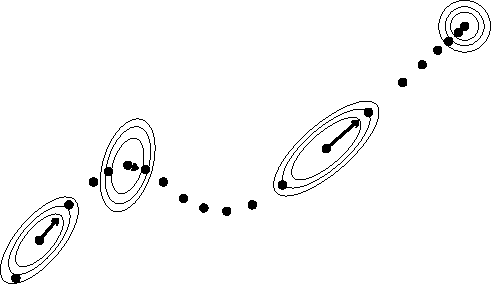
\includegraphics[width=.35\textwidth]{velocity_kernel}
    };
    
    \end{tikzpicture}
    \caption{Velocity-oriented anisotropic kernel.}
    \label{fig:kernel_anis}
\end{figure}
The anisotropic velocity kernel is defined as
\begin{equation}
    k(\mathbf{x}_i,\mathbf{x}_j) = e^{-(\mathbf{x}_i-\mathbf{x}_j)^T \Sigma (\mathbf{x}_i-\mathbf{x}_j)},
    \label{eqn:kernel_anis}
\end{equation}
where the matrix $\Sigma$ is constructed as follow
\begin{equation*}
    \Sigma = U D U^T
\end{equation*}
\begin{equation*}
    U =
    \begin{bmatrix}
    | & | \\
    \left( \frac{\bm{f}(\mathbf{x}_i)}{\norm{\mathbf{f}(\mathbf{x}_i)}}\right) & \left( \frac{\mathbf{f}(\mathbf{x}_i)}{\norm{\mathbf{f}(\mathbf{x}_i)}}\right)_{\perp} \\
    | & |
    \end{bmatrix}
\end{equation*}
\begin{equation*}
    D =
    \begin{bmatrix}
    e^{-\lambda \frac{\mathbf{f}(\mathbf{x}_i)}{\mathbf{f}_{max}}} & 0 \\
    0 & e^{\lambda \frac{\mathbf{f}(\mathbf{x}_i)}{\mathbf{f}_{max}}}
    \end{bmatrix}
\end{equation*}


\bibliographystyle{plain}
\bibliography{references}
\end{document}
